\chapter{Introduction}

\section{Problem Statement}

%Explain the context of your essay topic, so that the
%topic itself appears motivated, natural and important.


%Paragraphs are separated by blank lines in the \LaTeX\ code, 
%and the line spacing, paragraph indentation,
%and paragraph spacing are set in the preamble for you, 
%according to AIMS house style.

%This is a textual citation \citet{shannon44}. And this is a parenthetical citation \citep{shannon44}. You probably want to use the latter more often.

%\begin{figure}[h]
%\psfrag{A}{$d^2$}
%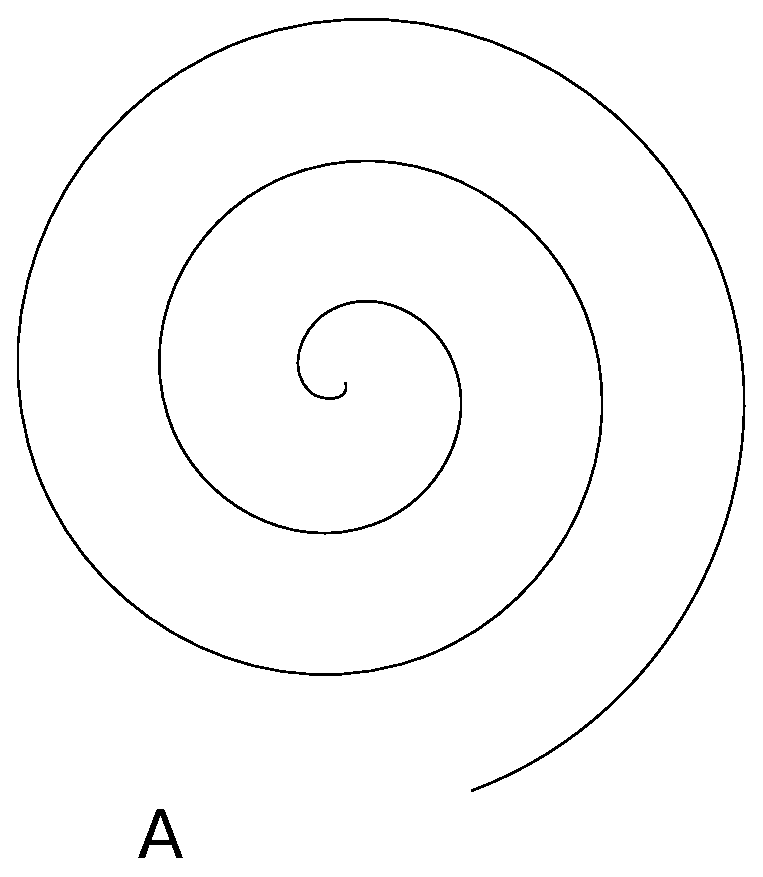
\includegraphics[scale=0.5]{images/drawing.eps}
%\end{figure}

Risk management is one of the fundamental tasks of insurance companies. The insurance industry should constantly adopt new technologies to address new risk types and trends affecting peoples lives.We depend on insurance for several reasons but it all scales down to the basic principle: minimizing risk in that clients pay a fee, and in exchange, insurers cover any costs that could arise with future calamities.

Clients provide extensive information to identify risk classification and illegibility, including scheduling medical exams, family medical history, credit history, behavioural risk factors, and so on, making the whole insurance process lengthy.The outcome is that the clients are turned off.This constitutes the main reason why majority of the households do not own individual life insurance.

Life underwriting has its own modelling challenges making insurers to turn to predictive  analytics to curb the problems.It is worth noting that auto underwriting has achieved remarkable success with predictive modelling unlike life underwriting where modelling is a new skill \citep{MikeBatty}. 

Building a predictive model requires:

\begin{enumerate}
\item[•] The availability of a sufficiently rich dataset where the predictive variables  correlate with the target can be identified

\item[•] An application by which results from the model are translated to business actions

\item[•] A clearly defined target variable

\item[•] A large number of observations to build the model so as surfacing relationships can be separated from random noise
\end{enumerate}

The above requirements are easily met with auto insurance.To clearly understand the challenges faced in life insurance, we compare life underwriting and auto underwriting.

\begin{enumerate}

\item[•] Auto insurers can make underwriting corrections if mistakes are made through rate increases in subsequent renewals of policies whereas life insurers must price policies appropriately from the outset

\item[•] For the auto insurer, the amount of insurance loss of a six-month contract is a target variable for the model. Life insurance is sold through long duration contracts, usually over a period of 10, 20 or more years.Due to the fact that the contribution of a given risk factor to mortality could change with time, it is not sufficient to analyse mortality experience over a short period of time

\item[•] Accessing historical data that can be used in modelling life insurance is a challenge.Not all life insurers record underwriting data in an electronic format; The available underwriting data that has been implemented in recent years is not available electronically or in a machine readable form. Even when such data has been captured for years, the content of the older data may be different from the data gathered for current applicants

\item[•] Life underwriting is subject to psychological biases and inconsistencies of human decision-making thus predictive models help to curb this challenge

\item[•] Life insurance claims have low frequency compared to auto insurance claims. Modelling statistically significant variation in either auto claims or mortality requires a large sample of loss events. Therefore auto insurers have ample data to build robust models using loss data while life insurers will find the data recorded in at similar times frames insufficient for modelling

Given that the target variable and data volume in life insurance is a concern, insurers are utilizing underwriting decisions as the target variable as they contain a lot of information, expert judgement, do not require long developing periods as in insurance claims and are abundant in supply.
\end{enumerate}

\section{Objective}
I am working on data from Prudential Life Insurance where the challenge is trying to make purchasing of life insurance easier by developing a predictive model that accurately classifies risk using a more automated approach. The data i am working on is from kaggle which is a platform for data science competitions. The host provides raw data and a description of the problem. Those participating in the competition then train algorithms where highly performing models can be adopted for predicting similar trends in the future.

\section{Trends in Insurance}
%Let's demonstrate a figure by looking at Fig.~\ref{bandwidth}. 
%
%\begin{figure}[!h]
% Use "\centering" in floats (figure, table), but if you need to center
% some text (why?) use "\begin{center}...\end{center}".
%\centering 
% Figure environments same as 0.8 * \textwidth please
% That does not necessarily mean the actual picture size,
% it is a guideline for the environmaRemember how to include code with {\tt verbatim} 
%and to fix the tabs in {\sf python} in a verbatim environment? 
%It may be best to have an `include' command for code, 
%not to have to re-edit it all the time.
%\verbatimtabinput{code/mycode.py}ndent which could contain
% 2 or more pictures! Be consistent and follow the guidelines
% provided in your sources.
%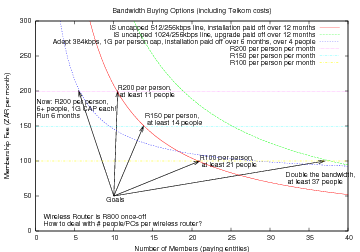
\includegraphics[width=0.8\textwidth]{images/bandwidth-colour.png}
%\caption{Planning community bandwidth sharing costs. 
%  Note caption capitalization.}
%\label{bandwidth} 
% if you move the label it breaks the reference numbering; 
% always have it *after* the caption.
%\end{figure}
 
%Remember how to include code with {\tt verbatim} 
%and to fix the tabs in {\sf python} in a verbatim environment? 
%It may be best to have an `include' command for code, 
%not to have to re-edit it all the time.
%\verbatimtabinput{code/mycode.py}

\textbf{Underwriting}

This is the process of understanding and evaluating risk in insuring a life or property.This ability is gained not only through theoretical study but also as a result of years of experience dealing with similar risks and mastering the art of paying claims on those risks. It is the traditional way of pricing and classifying risks in insurance \citep{macedo2009role}.

\citep{dickson2013actuarial} An insurance life office will have a premium rate schedule for a given type of policy.This rates depend on \textbf{the size of the policy and rating factors}.To establish an applicants risk level, a proposal form giving information on relevant rating factors such as age, gender,  any dangerous hobbies, occupation, smoking habits, and health history is filled. The purpose of underwriting is to classify potential policy holders into homogeneous risk categories and assess what additional premium would be appropriate if risk factors indicate that standard premium rates would be too low.


\textbf{Disadvantages}
\begin{enumerate}
\item[•] There is the risk of \textbf{adverse selection} by policy holders if the underwriting is not strict. This means that very high-risk individuals will buy insurance in disproportionate numbers leading to excessive losses.

\item[•] The underwriting process could be lengthy and costly

\item[•] Both the insurer and policy holder may assume 'utmost good faith' such that in case of loss and important information was held back or false,then the full sum assured may not be paid by the insurer in case the client claims from the insurance.
\end{enumerate}

Thus, the use of predictive models makes the underwriting process faster, more economical, more efficient and more consistent when the model is used to analyze a set of underwriting requirements.It is also worth noting that models are not subject to bias in the same way that underwriters ,who do not always act with perfect consistency or optimally weigh disparate pieces of evidence, are.

\section{Overview of Predictive Modelling}

In predictive modelling, two situations arise:

\begin{enumerate}
\item[•] One is required to fit a well-defined parametrized model to the data using a learning algorithm that can find parameters on the large dataset without over-fitting. In this case, lasso and elastic-net regularized generalised linear models are a set of modern algorithms which meet this need because they are fast, work on huge datasets and avoid over-fitting automatically.

\item[•] One needs to accurately predict a dependent variable. A learning algorithm that automatically identifies the structures, interactions and relationships in the data is needed. In this case, ensembles of decision trees (known as 'Random Forests') have been the most successful algorithm in modern times and basically this is what my work entails.
\end{enumerate}

\citep{berry1997data} Learning problems can be roughly categorized as either supervised or unsupervised.

\textbf{Supervised learning}: For each observation of the predictor measurement(s) $x_{i},i=1,2,...,n$, there is an associated response measurement $y_{i}$. We wish to find a model that relates the response to the predictors, with the aim of accurately predicting the response for future observations(predictions) and understand the relationship between the response and the predictors.Traditional statistical learning methods such as linear regression and logistic regression as well as modern approaches such as boosting and support vector machines work in the supervised learning domain.

\textbf{Unsupervised learning}: For every observation $i=1,2,...,n$, we observe a vector of measurements $x_{i}$ but no associated response $y_{i}$. A linear regression model cannot be fit because there is no response variable to predict.In this case we seek to find the relationship between the variables. One statistical tool that can be used is cluster analysis. Clustering ascertains whether the observations fall into distinct groups.

Supervised learning can be grouped into \textbf{Regression} and \textbf{Classification} problems.)

\begin{center}
\textbf{Regression Vs Classification Problems}
\end{center}
Variables can be grouped into \textbf{quantitative} or \textbf{qualitative} or categorical. Quantitative variables take on numerical values eg height while qualitative variables take on values in one of the different classes eg gender.

Problems with a quantitative response are referred to as regression problems while those involving a qualitative response are referred to as classification problems. Predicting a qualitative response for an observation is called classifying the observation since it involves assigning the observation to a class. Three of the most widely-used classifiers: logistic regression, k-nearest neighbors and Linear Discriminant Analysis. More computer-intensive methods are trees, random forests, support vector machines and boosting \citep{james2014introduction}.

\textbf{Machine Learning}: This is a method of teaching computers to improve and make predictions based on data.It is teaching a program to react to and recognize patterns through analysis, self training, observation and experience.

In the classification setting, we have a set of training observations $(x_{1},y_{1}),...,(x_{n},y_{n})$ that we can use to build a classifier. We want our classifier to perform well not only on the training data, but also on test observation not used to train the classifier.Here, I introduce some of the most commonly used classifiers.

\begin{center}
\textbf{Logistic Regression}
\end{center}

Models the probability that $Y$, the dependent variable belongs to a particular category (one of two categories eg 'yes' or 'no').


\textbf{The model}

Modelling the relationship between $p(X)=pr(Y=1/X)$ and $X$. For convenience we use the generic coding 0 and 1 for the response. To use linear regression to represent this probabilities we have, $p(X)=\beta_{0}+\beta_{1}X$ which gives the left hand side of the logistic function. 

However,there is a problem with this approach in that predicting of values close to zero would yield negative probabilities and if we were to predict large values, we would get probabilities bigger than 1 which defies the law of probability that probability values should fall between 0 and 1.

To prevent this,we model $p(X)$ using the logistic function that gives outputs between 0 and 1 for all values of $X$. 

\begin{equation*}
p(X)=\dfrac{\exp(\beta_0+\beta_{1}X)}{1+\exp(\beta_0+\beta_{1}X)}
\end{equation*}

We notice that for lower values, we now predict the probability of default as close to but never below $0$. Likewise for high values, we predict a default probability close to but, never above one.

Manipulating the equation gives;

\begin{equation}
\dfrac{p(X)}{1-p(X)}=\exp (\beta _0+\beta_{1}X)
\end{equation}

where the LHS is called odds and takes values between $0$ and $\infty$. Taking the logarithms on both sides yields:

\begin{equation}
log \left(\dfrac{p(X)}{1-p(X)}\right)=\beta_{0}+\beta_{1}X
\end{equation}

The LHS is called the log-odds or logit which is linear in $X$.

\begin{center}
\textbf{K-nearest Neighbors}
\end{center}

KNN can handle both binary and multi-class data.

Consider having $N$ training objects, each of which is represented by a set of attributes $X_{n}$ and a label $Y_{n}$.Suppose we want to classify new objects $X_{new}$, We first find the K training points closest to $X_{new}$. $Y_{new}$ is then set to be the majority class amongst these neighbors.

The figure below provides an illustrative example of the KNN approach \citep{james2014introduction}.

\begin{figure}[hbtp]
\caption{KNN approach using K=3.}
\centering
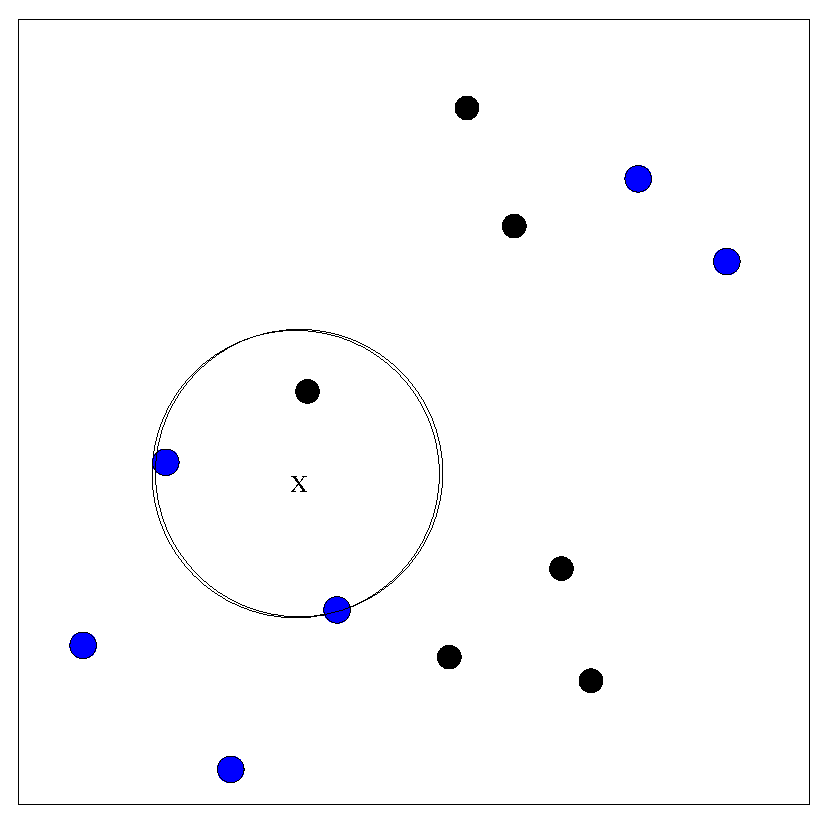
\includegraphics[scale=0.4]{KNN.eps}
\end{figure}


The goal is to predict the point labelled $X$. Suppose we choose $K=3$, KNN will first identify the three observations closest to $X$, as shown in the diagram. The point consists of two blue points and a red point resulting in estimated probabilities of $\dfrac{2}{3}$ for the blue class and $\dfrac{1}{3}$ for the black class. KNN will predict that the point $X$ belongs to the blue class.

\textbf{One draw back of KNN is the issue of ties}: Two or more classes having equal number of ties. Therefore,for binary classification,a good solution is to always use an odd number of neighbors.

\textbf{Choosing K}: If K is too small, the classification is heavily influenced by mislabelled points(noise). This problem is rectified by increasing K which regularises the boundary.

What about if K is too big? As we increase K, we are using neighbours further away from $X_{new}$ which is useful upto a certain point as it has a regularizing effect that reduces the chances of over-fitting.However, when we go too far, we loose the true pattern of the data we are attempting to model.Therefore, to find the best value of K, we use cross validation.

\begin{center}
\textbf{Linear Discriminant Analysis}
\end{center}

Linear Discriminant Analysis is used:
\begin{enumerate}
%\item[•] The parameter estimates for the logistic regression model are stable when the classes are well separated. LDA does not suffer from this problem.

\item[•] LDA is popular when we have more than two response classes.
\end{enumerate}

\textbf{Using bayes' theorem for classification}

Suppose we wish to classify an observation into K classes, where $K\geqslant 2$ and the qualitative response variable $Y$ can take on K distinct ordered values.

$\pi_{k}$: Denotes the prior probability that a randomly chosen observation comes from  class K of the response variable $Y$.

$f_{k}=Pr(X=x/Y=k)$: Denote the density function of X for an observation from class K.

Bayes theorem states that:

\begin{equation}
P_{k}(X)=Pr(Y=k/X=x)=\dfrac{\pi_{k}f_{k}(x)}{\sum \pi_{i}f_{i}(x)} \label{1.3.3}
\end{equation} 

$P_{k}(x)$: Posterior probability that an observation $X=x$ belongs to class K.

$\pi_{k}$ is computed if we have a random sample of $Y_{s}$ from the population. We therefore compute the fraction of training observations that belong to class K.$f_{k}(x)$ is estimated so we can develop a classifier that approximates the bayes classifier.

\begin{center}
Linear Discriminant Analysis for $p=1$.(We  have only one predictor)
\end{center}

We are required to find an estimate for $f_{k}(x)$ that we can plug into \eqref{1.3.3} inorder to estimate $p_{k}(x)$. We then classify an observation to the for which $p_{k}(x)$ is greatest. To estimate $f_{k}(x)$ the following assumptions are made:

\begin{enumerate}
\item[•] $f_{k}(x)$ is normal.
\begin{equation}
f_{k}(x)=\dfrac{1}{\sqrt{2 \pi}\sigma_{k}} \exp \left(-\dfrac{1}{2 \sigma^2_{k}}(x-\mu_{k})^2\right) \label{1.3.4}
\end{equation}

$\mu_{k}$ and $\sigma_{k}^2$ are the mean and variance parameters for class k.

\item[•] Shared variance term across all K classes, $\sigma_{1}^2=,...,=\sigma_{K}^2$
\end{enumerate}

Plugging equation \eqref{1.3.4} to equation \eqref{1.3.3} yields:

\begin{equation}
p_{k}(x)=\dfrac{\pi_{k}\dfrac{1}{\sqrt{2 \pi}\sigma} \exp \left(-\dfrac{1}{2 \sigma^2}(x-\mu_{k})^2\right)}{\sum_{i=1}^{K} \pi_{i}\dfrac{1}{\sqrt{2 \pi}\sigma} \exp \left(-\dfrac{1}{2 \sigma^2}(x-\mu_{i})^2\right)} \label{1.3.5}
\end{equation}

Taking the logs of equation \eqref{1.3.5} and rearranging the terms gives:

\begin{equation}
\delta_{k}(x)=x \dfrac{\mu_{k}}{\sigma^2}-\dfrac{\mu^2_{k}}{2 \sigma^2}+log(\pi_k) \label{1.3.6}
\end{equation}

It is not possible to calculate the bayes  classifier in real-life. We still need to estimate the parameters $\mu_{1},...,\mu_{K}, \pi_{1},...,\pi_{K}$ and $\sigma^2$. LDA method approximates the bayes classifier by plugging the estimates for $\pi_{k}, \mu_{k}$ and $\sigma^2$ into equation \eqref{1.3.6}.

The following estimates are used:

\begin{align}
\hat{\mu_k}&=\dfrac{1}{n_{k}} \sum _{i:y_i=k} x_{i}\\ \label{1.3.7}
\hat{\sigma}&=\dfrac{1}{n-K} \sum _{K=1}^K \sum _{i:y_i=k}(x_{i}-\hat{\mu})^2\\ \label{1.3.8}
\end{align}

$n$: Number of training observations
$n_k$: Total number of training observations in class k where $\mu_k$ is the average of all training observations from class k.

$\hat{\sigma}^2$: Weighted average of the sample variances for each of the k classes.

In the case where additional information is not present, LDA estimates $\pi_{k}$ using the proportion of training observations that belongs to the $k^{th}$ class.

\begin{equation}
\pi_{k}=\dfrac{n_k}{n} \label{1.3.9}
\end{equation}

LDA classifier plugs the estimates equation \eqref{1.3.7} and equation \eqref{1.3.8} into equation \eqref{1.3.6}, assigning an observation $X=x$ to the class for which 

\begin{equation}
\hat{\delta}_{k}(x)=x \dfrac{\hat{\mu_{k}}}{\hat{\sigma}^2}-\dfrac{\hat{\mu}^2_{k}}{2 \hat{\sigma}^2}+log(\hat{\pi}_k)
\end{equation}
is largest.

The classifier is linear due to the fact that the discriminant functions $\hat{\delta}_{k}(x)$ are linear functions of $x$.

I will use random forest for my analysis which i will discuss in depth in the subsequent chapter.